% generated by python -m specbridge.report.datamap_tex; do not edit
% Data map: sources (top), data built from them (middle), experiments with their sample sizes (bottom).
% Shared setup for the diagrams (teaser, pipeline, worked). Built with XeLaTeX so that all text is Arial, in black.
% Sizes match the paper's acmart sigconf sizes (\footnotesize 7 pt); the smallest text is 6 pt.
\documentclass[border=0.5pt]{standalone}
\usepackage{fontspec}
\setmainfont{Arial}\setsansfont{Arial}\setmonofont{Menlo}[Scale=MatchLowercase]
\usepackage{unicode-math}\setmathfont{FiraMath-Regular.otf}
\usepackage{booktabs}
\usepackage{tikz}
\usetikzlibrary{arrows.meta,calc,positioning,fit,backgrounds,shapes.geometric}
\renewcommand\large{\fontsize{10}{12}\selectfont}
\renewcommand\small{\fontsize{8}{10}\selectfont}
\renewcommand\footnotesize{\fontsize{7}{8.4}\selectfont}
\renewcommand\scriptsize{\fontsize{6.5}{7.6}\selectfont}
\renewcommand\tiny{\fontsize{6}{7}\selectfont}
\newcommand{\nohyph}{\hyphenpenalty=10000\exhyphenpenalty=10000\relax}
\newcommand{\sql}[1]{\texttt{#1}}
% the edited SQL clause, highlighted as in AMBROSIA and the test-suite paper; plain check and cross marks
\newcommand{\hl}[2]{{\setlength{\fboxsep}{0.7pt}\colorbox{#1f}{\vphantom{Ay}\texttt{#2}}}}
\newfontfamily\markfont{Arial Unicode MS}\newcommand{\yes}{{\markfont ✓}}\newcommand{\no}{{\markfont ✗}}
% math letters in Arial italic; the open-request circle is drawn; only the arrow comes from Fira Math
\newcommand{\vq}[1]{\textit{q}\textsubscript{#1}}\newcommand{\vp}[1]{\textit{p}\textsubscript{#1}}\newcommand{\vo}{\mbox{\textit{q}\hspace{0.3pt}\raisebox{-0.25ex}{\tikz[baseline=0pt]\draw[line width=0.45pt] (0,1.1pt) circle (1.1pt);}}}
% box lines: A (blue) and B (orange) as in the data figures; neutral lines grey. Text is always black.
% colors as in AMBROSIA's and AmbiQT's diagrams (draw.io palette): interpretation A blue, interpretation B orange, code blocks light gray
\definecolor{sbA}{HTML}{6C8EBF}\definecolor{sbB}{HTML}{D79B00}\definecolor{sbAf}{HTML}{DAE8FC}\definecolor{sbBf}{HTML}{FFE6CC}\definecolor{sbline}{HTML}{4D4D4D}
\definecolor{sbfill}{HTML}{F5F5F5}

\begin{document}
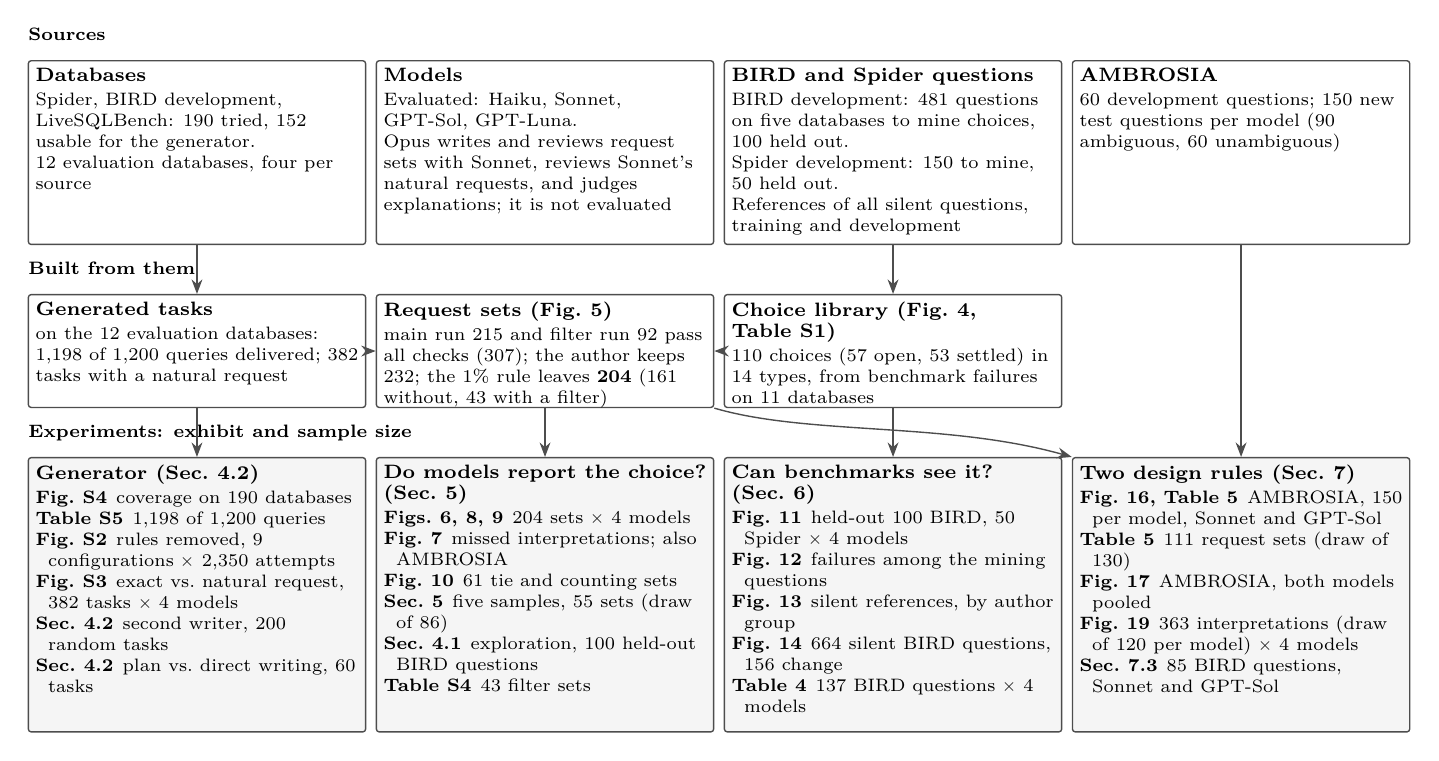
\begin{tikzpicture}[x=1cm, y=1cm, font=\scriptsize, >=Stealth, line width=0.5pt,
  bx/.style={execute at begin node=\nohyph, draw=sbline, rounded corners=1pt, inner sep=2.6pt, align=left, anchor=north west},
  ex/.style={bx, fill=sbfill},
  band/.style={font=\scriptsize\bfseries, anchor=north west, inner sep=0pt},
  arr/.style={->, draw=sbline}]
\newcommand{\hd}[1]{\textbf{\footnotesize #1}\\[1pt]}
\coordinate (r1) at (0,0);
\node[band] at (0,0.42) {Sources};
\node[bx] (dbs) at (0.00,0 |- r1) {\parbox[t][2.15cm][t]{4.10cm}{\nohyph\raggedright\hd{Databases}Spider, BIRD development, LiveSQLBench: 190 tried, 152 usable for the generator.\\12 evaluation databases, four per source}};
\node[bx] (qs) at (8.84,0 |- r1) {\parbox[t][2.15cm][t]{4.10cm}{\nohyph\raggedright\hd{BIRD and Spider questions}BIRD development: 481 questions on five databases to mine choices, 100 held out.\\Spider development: 150 to mine, 50 held out.\\References of all silent questions, training and development}};
\node[bx] (amb) at (13.26,0 |- r1) {\parbox[t][2.15cm][t]{4.10cm}{\nohyph\raggedright\hd{AMBROSIA}60 development questions; 150 new test questions per model (90 ambiguous, 60 unambiguous)}};
\node[bx] (mod) at (4.42,0 |- r1) {\parbox[t][2.15cm][t]{4.10cm}{\nohyph\raggedright\hd{Models}Evaluated: Haiku, Sonnet, GPT-Sol, GPT-Luna.\\Opus writes and reviews request sets with Sonnet, reviews Sonnet's natural requests, and judges explanations; it is not evaluated}};
\coordinate (r2) at ($(0,0 |- current bounding box.south)+(0,-0.62)$);
\node[band] at ($(r2)+(0,0.42)$) {Built from them};
\node[bx] (gen) at (0.00,0 |- r2) {\parbox[t][1.25cm][t]{4.10cm}{\nohyph\raggedright\hd{Generated tasks}on the 12 evaluation databases: 1,198 of 1,200 queries delivered; 382 tasks with a natural request}};
\node[bx] (rs) at (4.42,0 |- r2) {\parbox[t][1.25cm][t]{4.10cm}{\nohyph\raggedright\hd{Request sets (Fig.~5)}main run 215 and filter run 92 pass all checks (307); the author keeps 232; the 1\% rule leaves \textbf{204} (161 without, 43 with a filter)}};
\node[bx] (lib) at (8.84,0 |- r2) {\parbox[t][1.25cm][t]{4.10cm}{\nohyph\raggedright\hd{Choice library (Fig.~4, Table~S1)}110 choices (57 open, 53 settled) in 14 types, from benchmark failures on 11 databases}};
\coordinate (r3) at ($(0,0 |- current bounding box.south)+(0,-0.62)$);
\node[band] at ($(r3)+(0,0.42)$) {Experiments: exhibit and sample size};
\node[ex] (e1) at (0.00,0 |- r3) {\parbox[t][3.30cm][t]{4.10cm}{\nohyph\raggedright\hd{Generator (Sec.~4.2)}\hangindent=0.7em\hangafter=1 \textbf{Fig.~S4}\enspace coverage on 190 databases\par\hangindent=0.7em\hangafter=1 \textbf{Table~S5}\enspace 1,198 of 1,200 queries\par\hangindent=0.7em\hangafter=1 \textbf{Fig.~S2}\enspace rules removed, 9 configurations $\times$ 2,350 attempts\par\hangindent=0.7em\hangafter=1 \textbf{Fig.~S3}\enspace exact vs.\ natural request, 382 tasks $\times$ 4 models\par\hangindent=0.7em\hangafter=1 \textbf{Sec.~4.2}\enspace second writer, 200 random tasks\par\hangindent=0.7em\hangafter=1 \textbf{Sec.~4.2}\enspace plan vs.\ direct writing, 60 tasks\par}};
\node[ex] (e2) at (4.42,0 |- r3) {\parbox[t][3.30cm][t]{4.10cm}{\nohyph\raggedright\hd{Do models report the choice? (Sec.~5)}\hangindent=0.7em\hangafter=1 \textbf{Figs.~6, 8, 9}\enspace 204 sets $\times$ 4 models\par\hangindent=0.7em\hangafter=1 \textbf{Fig.~7}\enspace missed interpretations; also AMBROSIA\par\hangindent=0.7em\hangafter=1 \textbf{Fig.~10}\enspace 61 tie and counting sets\par\hangindent=0.7em\hangafter=1 \textbf{Sec.~5}\enspace five samples, 55 sets (draw of 86)\par\hangindent=0.7em\hangafter=1 \textbf{Sec.~4.1}\enspace exploration, 100 held-out BIRD questions\par\hangindent=0.7em\hangafter=1 \textbf{Table~S4}\enspace 43 filter sets\par}};
\node[ex] (e3) at (8.84,0 |- r3) {\parbox[t][3.30cm][t]{4.10cm}{\nohyph\raggedright\hd{Can benchmarks see it? (Sec.~6)}\hangindent=0.7em\hangafter=1 \textbf{Fig.~11}\enspace held-out 100 BIRD, 50 Spider $\times$ 4 models\par\hangindent=0.7em\hangafter=1 \textbf{Fig.~12}\enspace failures among the mining questions\par\hangindent=0.7em\hangafter=1 \textbf{Fig.~13}\enspace silent references, by author group\par\hangindent=0.7em\hangafter=1 \textbf{Fig.~14}\enspace 664 silent BIRD questions, 156 change\par\hangindent=0.7em\hangafter=1 \textbf{Table~4}\enspace 137 BIRD questions $\times$ 4 models\par}};
\node[ex] (e4) at (13.26,0 |- r3) {\parbox[t][3.30cm][t]{4.10cm}{\nohyph\raggedright\hd{Two design rules (Sec.~7)}\hangindent=0.7em\hangafter=1 \textbf{Fig.~16, Table~5}\enspace AMBROSIA, 150 per model, Sonnet and GPT-Sol\par\hangindent=0.7em\hangafter=1 \textbf{Table~5}\enspace 111 request sets (draw of 130)\par\hangindent=0.7em\hangafter=1 \textbf{Fig.~17}\enspace AMBROSIA, both models pooled\par\hangindent=0.7em\hangafter=1 \textbf{Fig.~19}\enspace 363 interpretations (draw of 120 per model) $\times$ 4 models\par\hangindent=0.7em\hangafter=1 \textbf{Sec.~7.3}\enspace 85 BIRD questions, Sonnet and GPT-Sol\par}};
% ---- arrows: what is built from what, and what each experiment uses
\draw[arr] (dbs.south) -- (gen.north);
\draw[arr] (qs.south) -- (lib.north);
\draw[arr] (gen.east) -- (rs.west);
\draw[arr] (lib.west) -- (rs.east);
\draw[arr] (gen.south) -- (e1.north);
\draw[arr] (rs.south) -- (e2.north);
\draw[arr] (lib.south) -- (e3.north);
\draw[arr] (amb.south) -- (e4.north);
\draw[arr] (rs.south east) .. controls +(1.2,-0.35) and +(-1.6,0.45) .. (e4.north west);
\end{tikzpicture}
\end{document}
